\documentclass[compress]{beamer}
\usepackage[
    title={Collaborative Learning},
    subtitle={Una soluzione di reinforcement learning applicata a un nodo router di messaggi},
    event={Progetto fine corso Machine Learning},
    author={DLP, MC, LF},
    longauthor={Daniele La Prova, Matteo Conti, Luca Falasca},
    email={},
    institute={ML 2023-2024},
    longinstitute={Universita' degli Studi di Roma Tor Vergata},
]{unislides}
\usepackage{graphicx} % Required for inserting images
\usepackage{minted}
\usepackage{algorithm}
\usepackage{hyperref}
\usepackage{adjustbox}
\usepackage{svg}
\svgsetup{inkscapelatex=false}

\begin{document}

\begin{frame}[plain]
    \titlepage
\end{frame}

\section{Introduzione}
%TODO:

\subsection{Contesto}
\begin{frame}{\subsecname\ (1)}
    In un sistema moderno i QoS possono essere di vario genere e non sempre sono legati alle sole prestazioni, in particolare, hanno acquisito sempre più rilevanza aspetti come la sostenibilità ed il valore portato dal sistema.\\ E' quindi necessario trovare delle soluzioni che siano flessibili rispetto a tali aspetti in modo da poter essere adattate a diversi contesti.
    \vspace{2cm}
    \begin{adjustbox}{margin=0.4cm 0cm 0cm 0.65cm, center} % left, bottom, right, top
        
\includegraphics[width=.6\textwidth]{figs/qos_adapt.png}
    \end{adjustbox}
\end{frame}

\begin{frame}{\subsecname\ (2)}
    Il progetto verte sulla realizzazione di un nodo di rete dotato di code di priorità e diverse fonti energetiche il cui comportamento è determinato da un agente di reinforcement learning che cerca di minimizzare una reward configurabile basata sui seguenti QoS:
    \begin{columns}
        \column{0.5\textwidth}
            \begin{minipage}[b]{1\textwidth}
                \begin{itemize}
                    \item Costo energetico
                    \item Occupazione delle code
                    \item Perdita di pacchetti dalle code 
                \end{itemize}
            \end{minipage}
            \column{0.5\textwidth}
                \begin{minipage}{1\textwidth}
                    \begin{adjustbox}{margin=0cm 0cm 0cm 0cm, center} % left, bottom, right, top
                        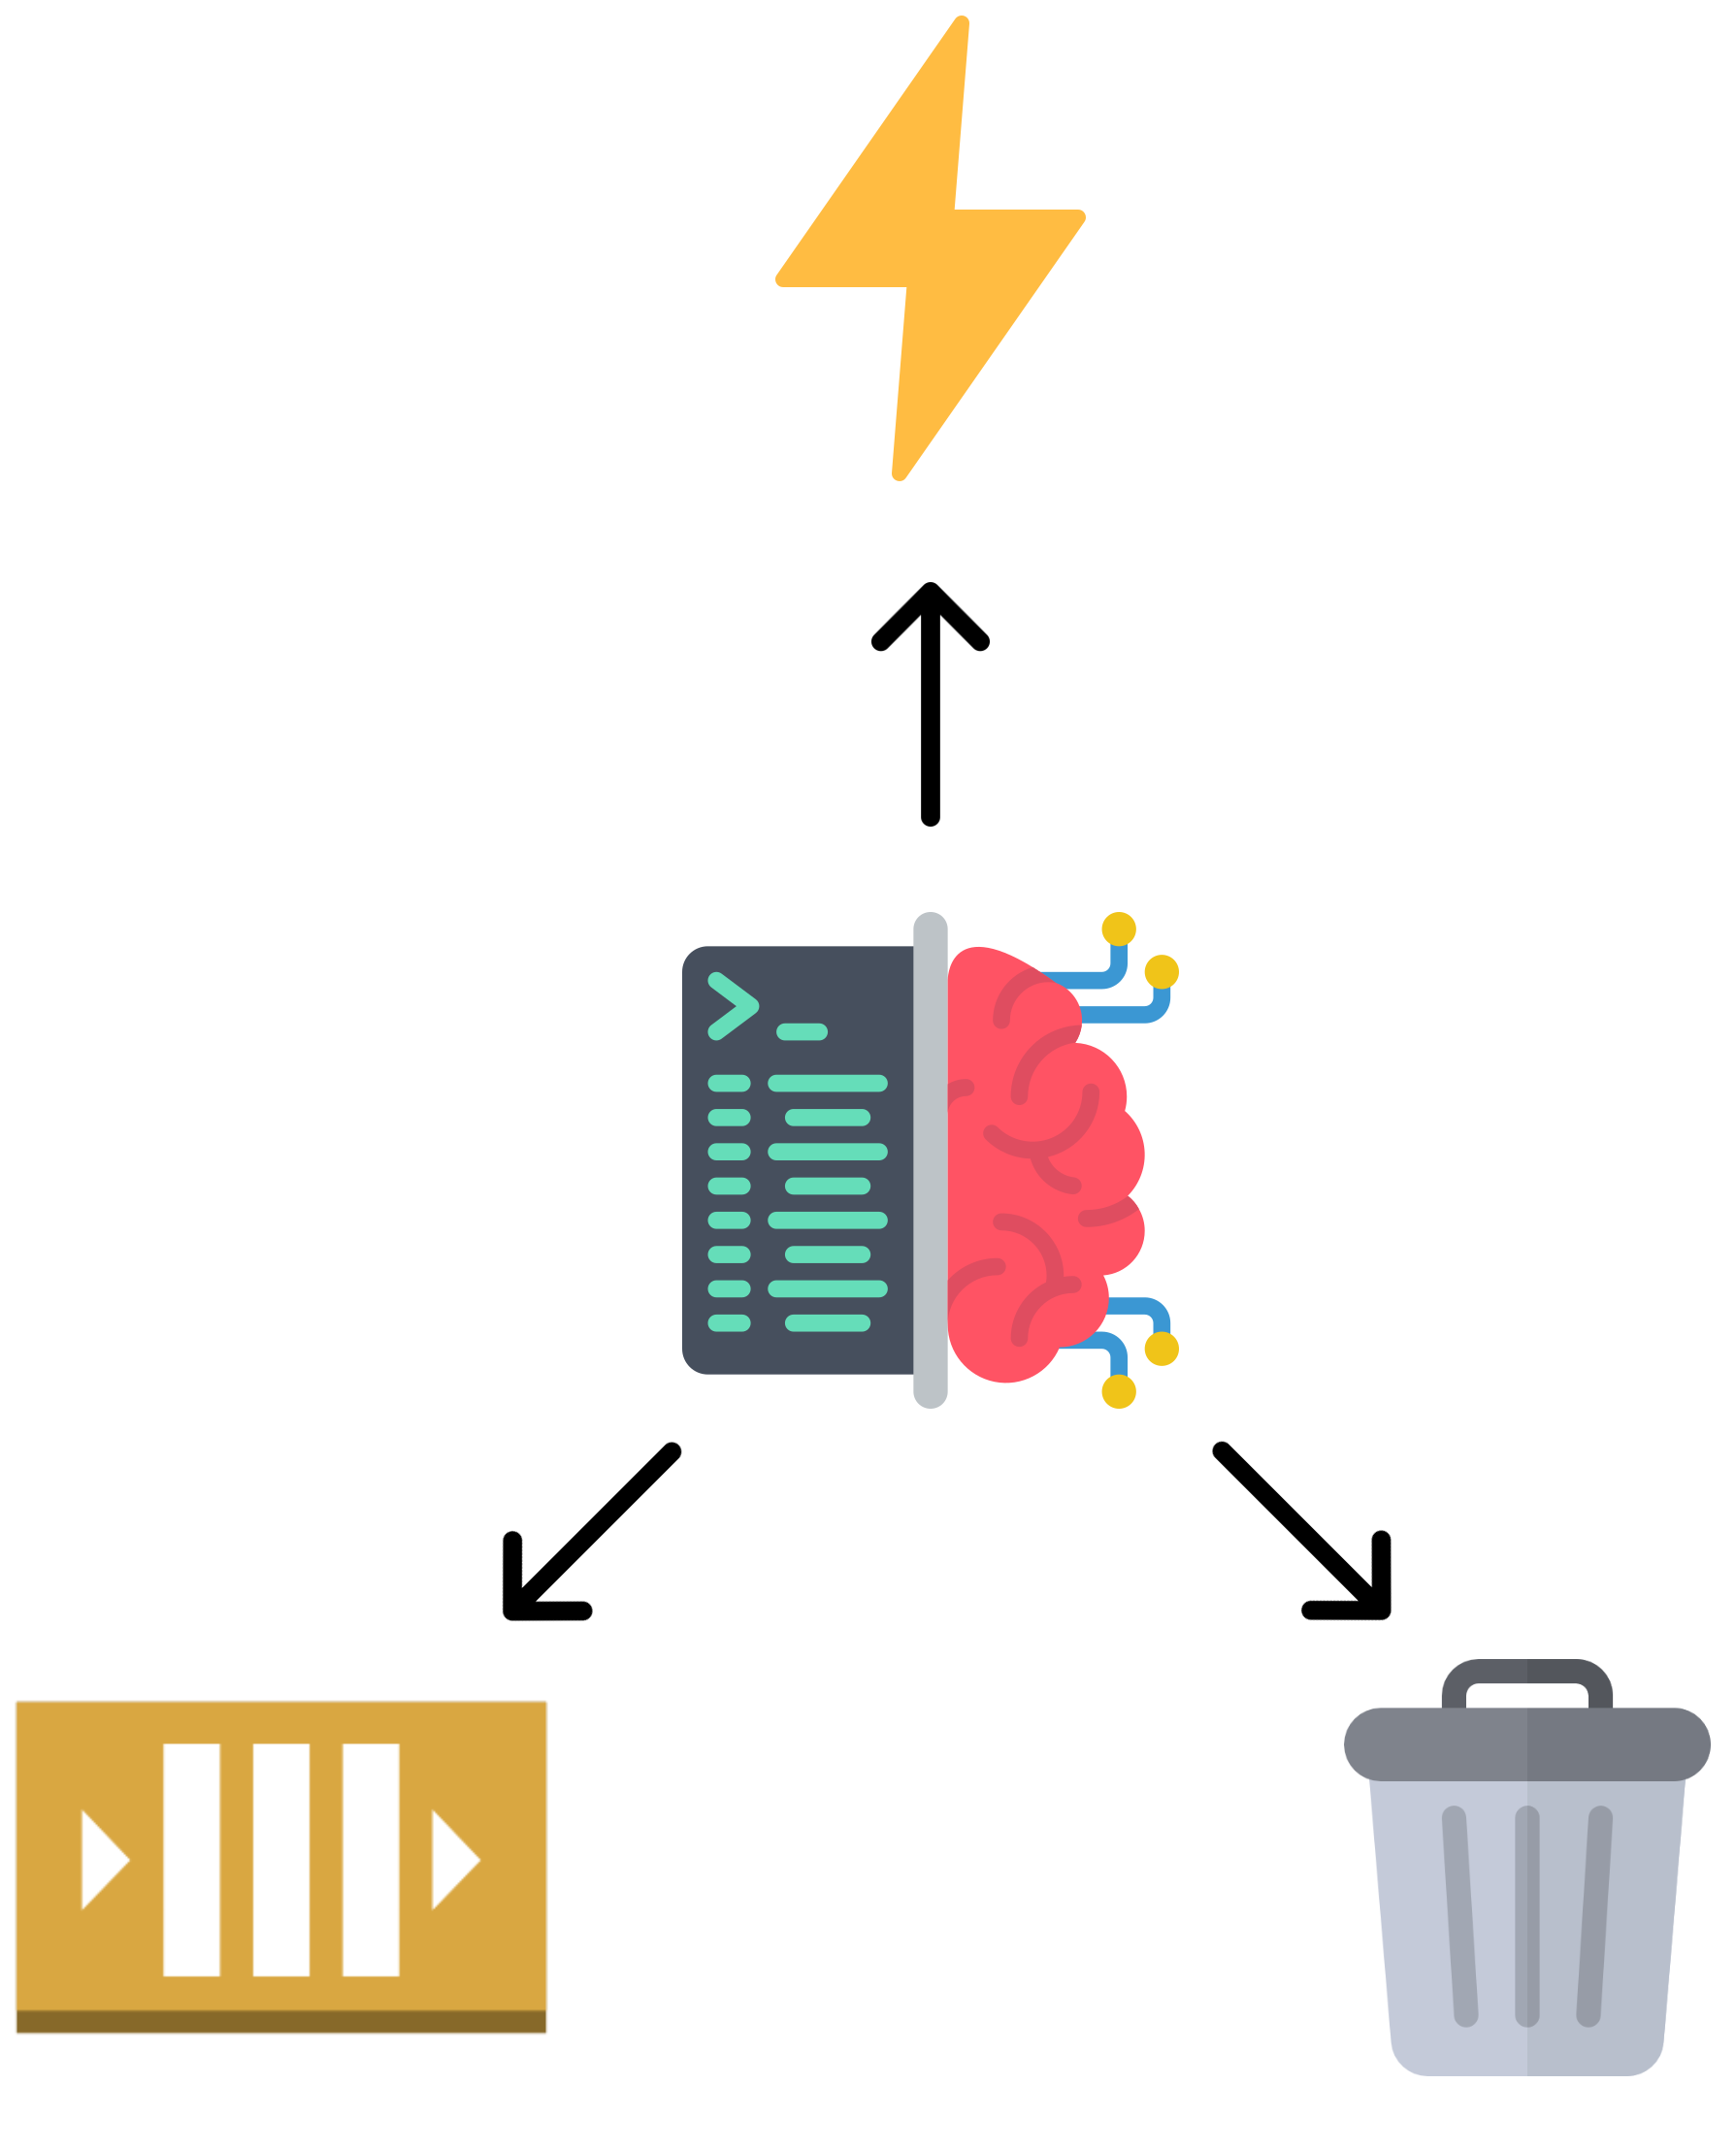
\includegraphics[width=.65\textwidth]{figs/agent_icon.png}
                    \end{adjustbox}
                \end{minipage}
    \end{columns}
\end{frame}
\subsection{Obiettivi}

\section{Metodologia}
\subsection{Modello}
\subsubsection{Stato}
\begin{frame}
    \frametitle{\subsecname: \subsubsecname}
    \begin{itemize}
        \item Per catturare lo stato della simulazione è stato deciso di campionare a ogni timestep le
        seguenti variabili:
        \begin{itemize}
            \item Percentuale di carica della batteria;
            \item Quanta percentuale di batteria è stata ricaricata nell'ultimo timestep;
            \item La percentuale di occupazione delle code, un valore per ogni coda. 
        \end{itemize}
        \item Tali valori sono stati discretizzati ove possibile per permetterne la comprensione da
        parte di alcune implementazioni di agenti, ad esempio il DQN.        
    \end{itemize}
\end{frame}

\subsubsection{Azioni}
\begin{frame}
    \frametitle{\subsecname: \subsubsecname}
    \begin{itemize}
        \item Un nodo può essenzialmente svolgere due operazioni in un qualunque timestep:
        \begin{itemize}
            \item Non fare nulla
            \item Inviare un pacchetto
        \end{itemize}
            \item Qualora l'azione scelta sia quella di inviare un pacchetto, allora è necessario anche
            scegliere:
        \begin{itemize}
            \item Da quale coda prelevare il pacchetto
            \item Da quale power source attingere l'energia necessaria per l'invio
        \end{itemize}
    \end{itemize}
\end{frame}

\subsubsection{Reward}
\begin{frame}
    \frametitle{\subsecname: \subsubsecname}
    \begin{Definition}[Reward per timestep]
        \begin{equation}
            \label{eq:reward}
            \begin{aligned}
                & r(t) = \sum_{i \in T} w_i \cdot r_i(t), & -1 \leq r_i \leq 0\\
                && 0 \leq w_i \leq 1, \\
                && \sum_{i \in T} w_i = 1, \\
                && T = \{e, o, d\},\\
                && t \geq 0 \in \mathbb{N}
            \end{aligned}
        \end{equation}
    \end{Definition}
    \only<+>{ \begin{itemize}
        \item La reward $r$ da inviare all'agente per un qualunque timestep $t$ è calcolata come la somma pesata dei contributi normalizzati del termine energetico,
        di occupazione delle code e di drop dei pacchetti in quel timestep
    \end{itemize}}
    \only<+> {\begin{itemize}
        \item Tutti i termini della reward sono confrontabili tra loro;
        \item configurando opportunamente i pesi è possibile costringere l'agente
        a minimizzare dei termini anche a discapito di altri
    \end{itemize}}
\end{frame}
\begin{frame}
    \frametitle{\subsecname: \subsubsecname}
    \begin{Definition}[Reward Power Term]
        \begin{equation}
            \label{eq:reward_energy}
            \begin{aligned}
                & r_e(t) = -\sum_{p \in P}\frac{\text{cons}_p(t) \cdot \text{cost}_p}{\max_{\tau < t}\{\text{cons}_p(\tau)\} \cdot \sum_{p \in P}\text{cost}_p},\\
                & P = \{\text{battery}, \text{power chord}\} 
            \end{aligned}
        \end{equation}
    \end{Definition}
    \begin{itemize}
        \item Il termine energetico per una power source è calcolato come il prodotto tra il consumo energetico della power source $p$ e il
        suo costo di utilizzo, normalizzato sul massimo consumo energetico registrato fino
        a quel time step per quella power source moltiplicato per la somma dei costi di utilizzo.
        \item i costi e i consumi energetici sono tutti maggiori di zero
    \end{itemize}
\end{frame}
\begin{frame}
    \frametitle{\subsecname: \subsubsecname}
    \begin{Definition}[Reward Queue Occupancy Term]
        \begin{equation}
            \label{eq:reward_occupancy}
            \begin{aligned}
                & r_o(t) = -\sum_{q \in Q}\frac{\text{occ}_q(t) \cdot p_q}{\max_{\tau < t}\{\text{occ}_q(\tau)\} \cdot \sum_{q \in Q}p_q},\\
                & Q = \{0, 1, \dots \#Q - 1\} 
            \end{aligned}
        \end{equation}
    \end{Definition}
    \begin{itemize}
        \item Il termine dell'occupazione di una coda è calcolato come il prodotto tra la percentuale di occupazione della coda $q$ nel 
        timestep $t$ e la sua priorità $p_q$, normalizzato sul massimo valore di occupazione
        registrato fino a quel time step per quella coda moltiplicato per la somma delle priorità.
        \item La priorità di una coda $p_q$ è data dal suo indice di coda $q + 1$ 
    \end{itemize}
\end{frame}
\begin{frame}
    \frametitle{\subsecname: \subsubsecname}
    \begin{Definition}[Reward Packet Drop Term]
        \begin{equation}
            \label{eq:reward_drop}
            \begin{aligned}
                & r_d(t) = -\sum_{q \in Q}\frac{\text{drop}_q(t) \cdot p_q}{\text{inbound}_q(t) \cdot \sum_{q \in Q}p_q},\\
                & Q = \{0, 1, \dots \#Q - 1\} 
            \end{aligned}
        \end{equation}
    \end{Definition}
    \begin{itemize}
        \item Il termine del drop dei pacchetti di una coda è calcolato come il prodotto tra il numero di pacchetti persi dalla coda $q$ nel 
        timestep $t$ e la sua priorità $p_q$, normalizzato sul numero di pacchetti arrivati alla coda in quel time step moltiplicato per la somma delle priorità.
    \end{itemize}
\end{frame}

\subsection{Agente}
%TODO:

\subsubsection{AgentFaçade}
%TODO:

\subsubsection{AgentFactory}
%TODO:

\subsubsection{Decisions}
%TODO:

\subsection{Simulazione}
\begin{frame}{\subsecname}
    Per la simulazione è stato utilizzato il framework OMNeT++, il quale permette di definire e simulare una rete di nodi. \\Dato che OMNeT++ non supporta nativamente Python per permettere la comunicazione tra l'agente ed il nodo, è stata utilizzata la libreria PyBind la quale permette di esporre simboli in Python e C++ e farne il binding.
    \begin{adjustbox}{margin=0cm 0cm 0cm 0.5cm, center} % left, bottom, right, top
        
\includegraphics[width=.8\textwidth]{figs/pybind_omnet.png}
    \end{adjustbox}
\end{frame}

\subsubsection{Nodo}
\begin{frame}{\subsubsecname}
    E' l'elemento della rete che è in grado di ricevere e inviare messaggi sulla base della scelta dell'agente, è composto da:
    \begin{columns}
        \column{0.5\textwidth}
            \begin{minipage}[b]{1\textwidth}
                \begin{itemize}
                    \item Controller, che implementa la logica del nodo
                    \item AgentClient, che permette la comunicazione con l'agente
                    \item Queues, una o più code che accodano messaggi
                \end{itemize}
            \end{minipage}
        \column{0.5\textwidth}
            \begin{minipage}{1\textwidth}
                \begin{adjustbox}{margin=0cm 0cm 0.1cm 0.2cm, center} % left, bottom, right, top
                    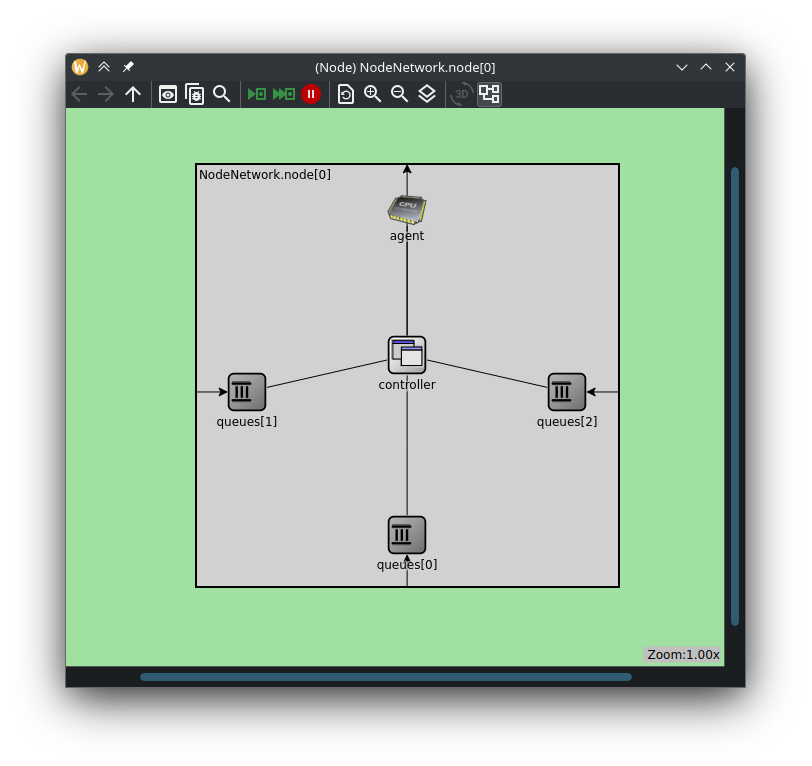
\includegraphics[width=1\textwidth]{figs/node_layout_3queues.png}
                \end{adjustbox}
            \end{minipage}
    \end{columns}
\end{frame}

\subsubsection*{Nodo - Controller}
\begin{frame}{\subsubsecname\ (1)}
E' il componente che implementa la logica del nodo, in particolare:
\vspace{0.5cm}
    \begin{columns}
        \column{0.6\textwidth}
            \begin{minipage}[b]{1\textwidth}
                \begin{itemize}
                    \item Campiona lo stato visibile al nodo
                    \item Interroga l'agente per ottenere l'azione consegnandogli la reward dell'azione precedente
                    \item Attua l'azione ricevuta dall'agente
                    \item Calcola la reward per le azioni ricevute dall'agente
                \end{itemize}
            \end{minipage}
        \column{0.4\textwidth}
            \begin{minipage}{.9\textwidth}
                \begin{adjustbox}{margin=0.5cm 0cm 0.1cm 0.2cm, center} % left, bottom, right, top
                    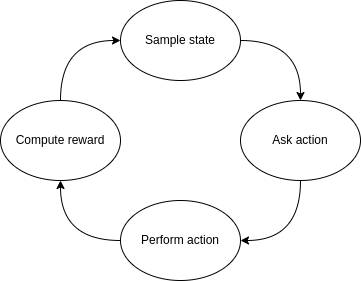
\includegraphics[width=1\textwidth]{figs/control_loop.png}
                \end{adjustbox}
            \end{minipage}
    \end{columns}
\end{frame}

\begin{frame}{\subsubsecname\ (2)}
    Il controller si occupa anche di gestire le sorgenti energetiche del nodo, in particolare:
    \vspace{0.5cm}
        \begin{columns}
            \column{0.6\textwidth}
                \begin{minipage}[b]{1\textwidth}
                    \begin{itemize}
                        \item una batteria,
                        avente un costo di utilizzo pari a zero ma una capacità limitata e una ricarica influenzata
                        da fattori ambientali;
                        \item Una presa di corrente, che ha un costo di utilizzo diverso
                        da zero ma una capacità pressoché illimitata.
                    \end{itemize}
                \end{minipage}
            \column{0.4\textwidth}
                \begin{minipage}{.9\textwidth}
                    \begin{adjustbox}{margin=0.5cm 0cm 0.1cm 0.2cm, center} % left, bottom, right, top
                        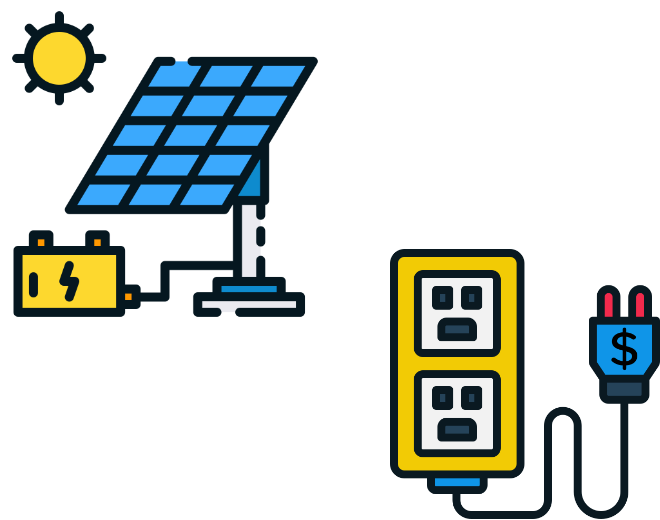
\includegraphics[width=1\textwidth]{figs/socket_battery.png}
                    \end{adjustbox}
                \end{minipage}
        \end{columns}
    \end{frame}

\subsubsection*{Nodo - Agent Client}
\begin{frame}{\subsubsecname}
    E' il componente che fa da intermediario tra il controller e l'Agente

    \begin{figure}
        \centering
        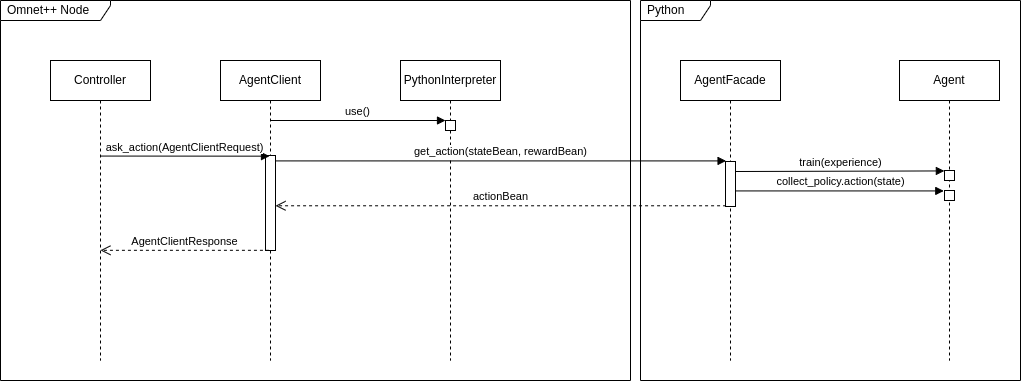
\includegraphics[width=\textwidth]{figs/agentc_sequence_diagram.drawio.png}
        \caption{sequence diagram per la servitura di una richiesta di azione del Controller nei confronti dell'agente.}
        \label{fig:agentc_sequence_diagram}
    \end{figure}
\end{frame}

\subsubsection*{Nodo - Queue}
\begin{frame}{\subsubsecname}
    E' il componente che implementa la logica della coda, in particolare:
    \vspace{0.5cm}
        \begin{columns}
            \column{0.6\textwidth}
                \begin{minipage}[b]{1\textwidth}
                    \begin{itemize}
                        \item Accoglie i pacchetti in arrivo, scartandoli se la coda è piena
                        \item Riceve le QueueDataRequest di pacchetti da parte del controller
                        \item Consegna i pacchetti al controller in delle QueueDataResponse
                        \item Comunica al controller gli aggiornamenti sullo stato della coda, tramite una QueueStateUpdate, ogni volta che arriva un pacchetto
                    \end{itemize}
                \end{minipage}
            \column{0.4\textwidth}
                \begin{minipage}{.9\textwidth}
                    \begin{adjustbox}{margin=0.5cm 0cm 0.1cm 0cm, center} % left, bottom, right, top
                        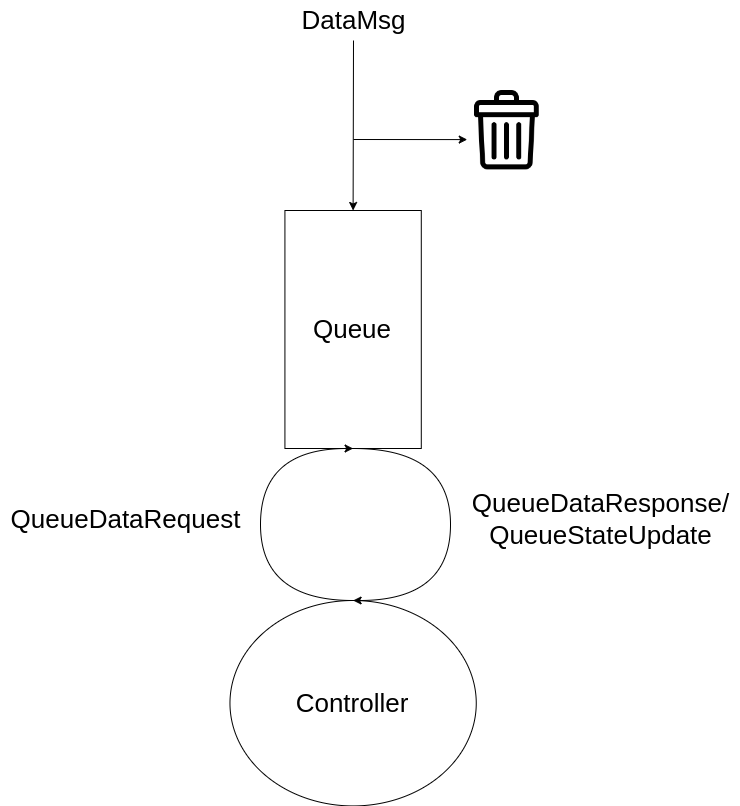
\includegraphics[width=1\textwidth]{figs/queue_scheme.png}
                    \end{adjustbox}
                \end{minipage}
        \end{columns}
\end{frame}

\subsubsection{SrcNode}
\begin{frame}{\subsubsecname}
    E' l'elemento della rete che si occupa di generare il traffico, ogni Queue ha associato un SrcNode.
    Il tempo di interarrivo dei pacchetti è regolato da una distribuzione esponenziale con tasso $\lambda$ configurabile, mentre la dimensione dei pacchetti è regolata da una distribuzione uniforme su un intervallo configurabile.
    \begin{adjustbox}{margin=0.5cm 0cm 0.5cm 0.5cm, center} % left, bottom, right, top
        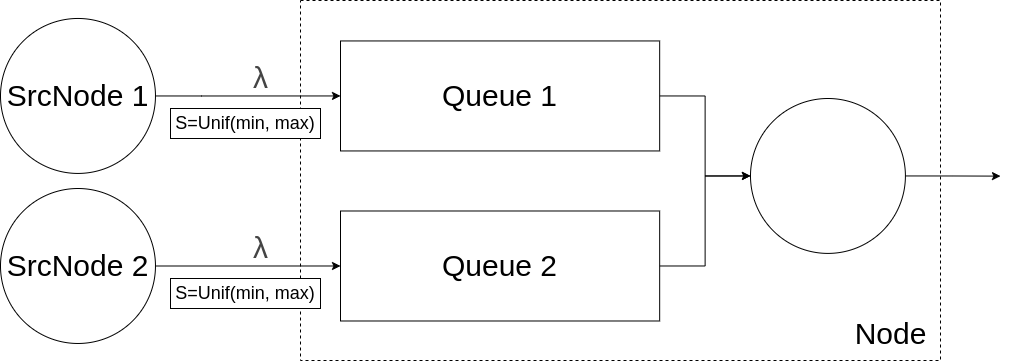
\includegraphics[width=.8\textwidth]{figs/src_scheme.png}
    \end{adjustbox}
\end{frame}

\subsubsection{Network}
\begin{frame}{\subsubsecname}
E' l'ambiente in cui vivono tutti gli elementi della simulazione, qui vengono specificati i collegamenti tra i SrcNode e le code del nodo router. 
    \begin{adjustbox}{margin=0cm 0cm 0cm 0cm, center} % left, bottom, right, top
        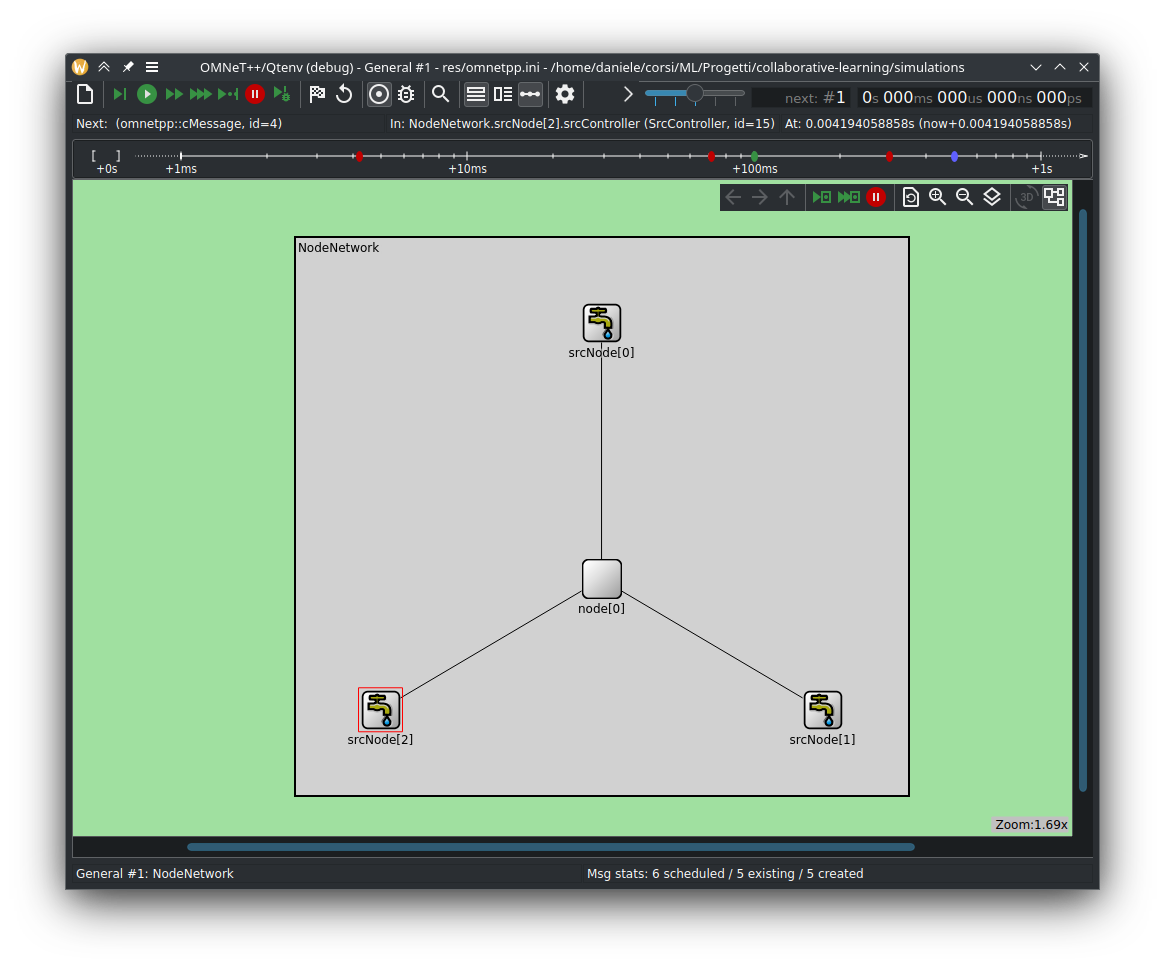
\includegraphics[width=.65\textwidth]{figs/network_layout_3queues.png}
    \end{adjustbox}
\end{frame}


\section{Risultati}
\begin{frame}
    \frametitle{\secname}
    \begin{itemize}
        \item Sono stati condotti diversi esperimenti per valutare le prestazioni del nodo in base 
        alle azioni suggerite dal suo agente
        \item Per effettuare gli esperimenti si è partiti da una configurazione dei parametri di 
        base\footnote{\href{https://github.com/retarded-reward/collaborative-learning/blob/main/simulations/res/omnetpp.ini}{https://github.com/retarded-reward/collaborative-learning/blob/main/simulations/res/omnetpp.ini}},
        a cui poi sono state apportate modifiche a seconda dello scenario considerato
        nell'esperimento.
        \item Negli esperimenti andiamo a confrontare tre tipologie di agenti:
        \begin{itemize}
            \item DQN: Agente DQN implementato secondo le specifiche delle Decisions
            \item DQN flat: Agente DQN in cui le azioni sono l'enumerazione di tutte
             le possibili azioni (Albero delle decisions con 1 singolo nodo). 
            \item Random: Agente che sceglie casualmente tra le azioni,
             utilizzato per avere un benchmark di confronto.
        \end{itemize}
    \end{itemize}
\end{frame}

\subsection{Coda singola, reward bilanciata}

\begin{frame}
    \frametitle{\secname: \subsecname}
    \begin{figure}
        \centering
        \includesvg[scale = 0.19]{figs/results_charts/cumulativeReward_default_allAgents.svg}
        \label{fig:cumulative_reward_dqnDeep_dqnFlat_random_defaultConfig}
    \end{figure}
    \begin{itemize}
        \item l'agente DQN sembra imparare una politica più vantaggiosa dopo
         50 secondi di simulazione
        \item Il DQN con decisions sembra
        imparare più lentamente rispetto al DQN flat, per poi peggiorare
    \end{itemize}
\end{frame}
\begin{frame}
    \frametitle{\secname: \subsecname}
    \begin{figure}
        \centering
        \includesvg[scale = 0.19]{figs/results_charts/sendCount_allAgents_defaultConfig.svg}
        \label{fig:sendCount_allAgents_defaultConfig}
    \end{figure}
    \begin{itemize}
        \item l'agente root sembra essere scoraggiato dall'inviare pacchetti a causa delle scelte di agenti
        più in profondità nell'albero delle decisions, ad esempio se l'agente responsabile della
        scelta della power source sceglie spesso di ricorrere al power chord.
    \end{itemize}
\end{frame}
\begin{frame}
    \frametitle{\secname: \subsecname}
    \begin{figure}
        \centering
        \includesvg[scale = 0.19]{figs/results_charts/energySaving_defaultConfig_allAgents.svg}
        \label{fig:energySaving_defaultConfig_allAgents}
        \end{figure}
    \only<+> {\begin{itemize}
        \item gli agenti DQN e DQN flat presentano un risparmio di spesa energetica più basso (6\%, 8\%) rispetto al Random (14\%)
        \item gli agenti DQN sembrano inviare più spesso pacchetti dalla power chord piuttosto che dalla batteria
    \end{itemize}}
    \only<+>{ \begin{itemize}
        \item  Ciò potrebbe essere dovuto al fallback dato che nello stato dell'agente non è presente alcuna informazione relativa al consumo energetico
    \end{itemize}}
\end{frame}
\begin{frame}
    \frametitle{\secname: \subsecname}
    \begin{figure}
        \centering
        \includesvg[scale = 0.19]{figs/results_charts/occupancies_allAgents_defaultConfig.svg}
        \label{fig:occupancies_allAgents_defaultConfig}
    \end{figure}
    \begin{itemize}
        \item gli agenti
        DQN e DQN flat riescano a gestire meglio la popolazione della coda rispetto al
        Random
        \item in certi periodi
        si concentrano nell'invio di pacchetti continuo, mentre in altri non fanno niente
    \end{itemize}    
\end{frame}
\begin{frame}
    \frametitle{\secname: \subsecname}
    \begin{figure}
        \centering
        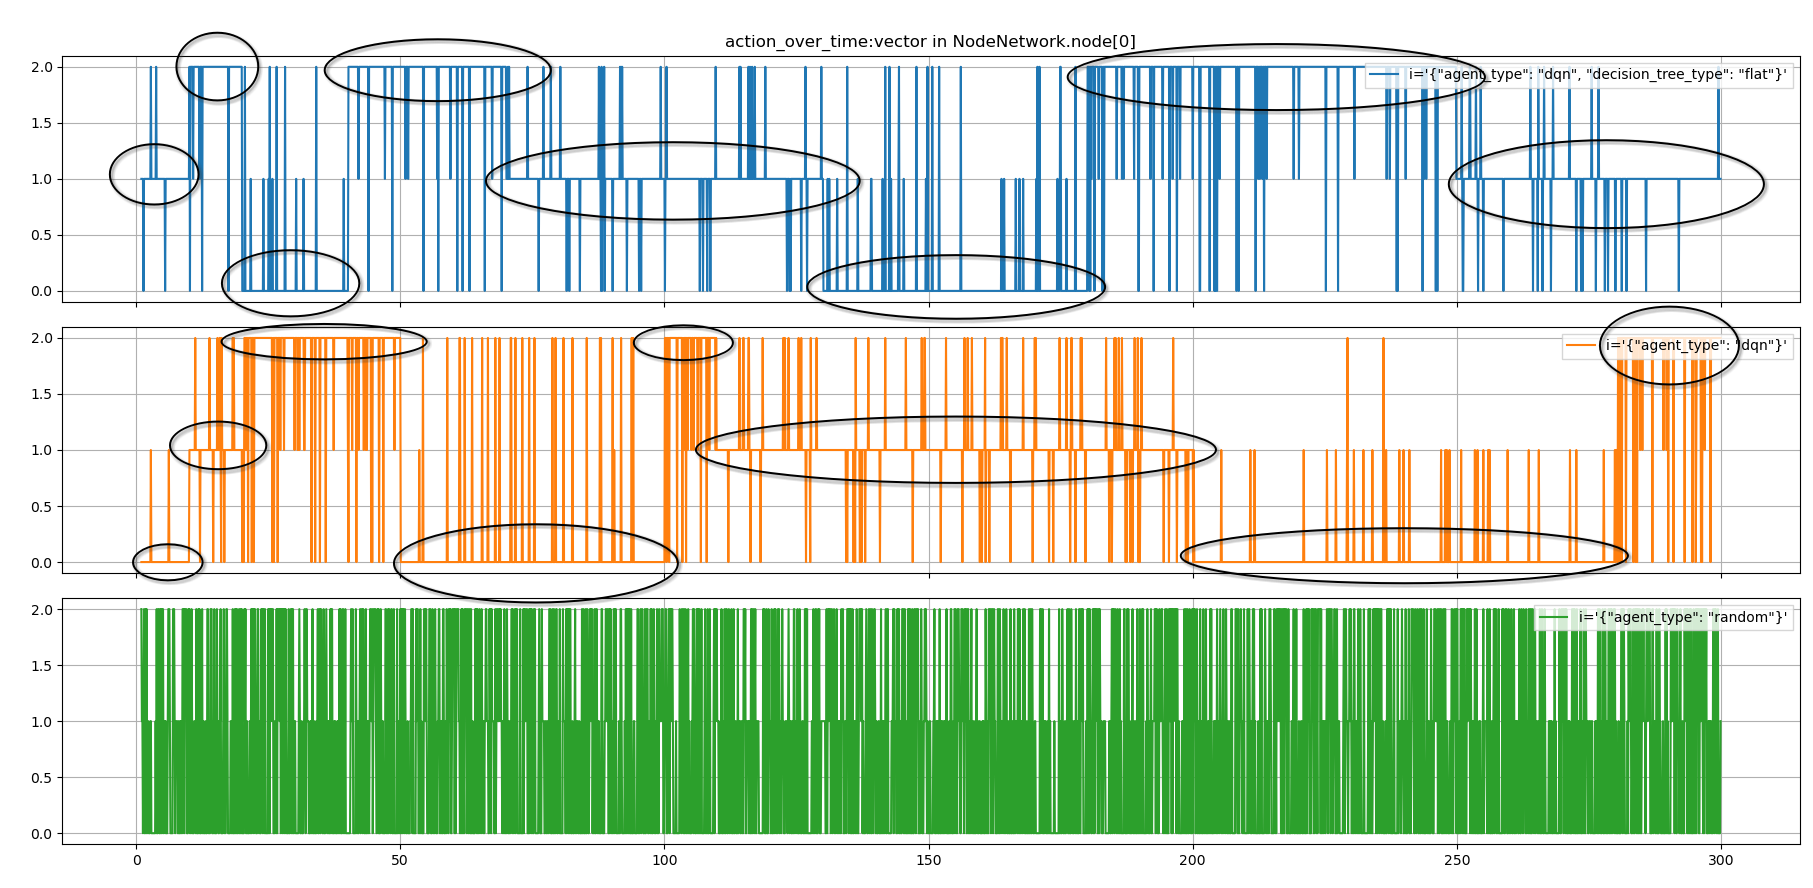
\includegraphics[scale = 0.24]{figs/results_charts/actionOverTime_allAgents_defaultConfig_annotated.png}
        \label{fig:actionOverTime_allAgents_defaultConfig_annotated}
        \end{figure}
    \begin{itemize}
        \item  il DQN con decision oscilla di meno rispetto alla versione flat, anche se
        accumula più reward negativa.
    \end{itemize}    
\end{frame}

\subsection{Coda singola, full power saving}
\begin{frame}
    \frametitle{\secname: \subsecname}
    \begin{figure}
        \includesvg[scale=0.19]{figs/results_charts/allPowerSaving_allAgents_defaultConfig.svg}
        \label{fig:allPowerSaving_allAgents_defaultConfig}
    \end{figure}    
    \begin{itemize}
        \item il DQN con decisions sembra 
        andare meglio rispetto alla controparte flat
        \item la decision root deve scegliere solo tra due azioni e quindi
        impara più in fretta che non conviene inviare mai rispetto al DQN flat
    \end{itemize}
\end{frame}

\subsection{Coda singola, no power saving}
\begin{frame}
    \frametitle{\secname: \subsecname}
    \begin{figure}
        \centering
        \includesvg[scale=0.19]{figs/results_charts/noPowerSaving_allAgents_defaultConfig.svg}
        \label{fig:noPowerSaving_allAgents_defaultConfig}
    \end{figure}
        \begin{itemize}
        \item le varianti di DQN accumulino un quantitivo di reward simile rispetto allo
        scenario con reward bilanciata, mentre il random va peggio.
        \item a pesare
        maggiormente sulla reward sono i termini riguardanti le code, e la
        strategia imparata dal DQN punta sempre a minimizzarli.
    \end{itemize}
\end{frame}
\subsection{3 Code, reward bilanciata}
\begin{frame}
    \frametitle{\secname: \subsecname}
    \begin{figure}
        \includesvg[scale=0.19]{figs/results_charts/balanced_allAgents_5queues_300s.svg}
        \label{fig:balanced_allAgents_5queues_300s}
    \end{figure}
        \begin{itemize}
        \item gli agenti 
        DQN hanno un comportamento peggiore del random, segno che non sono riusciti a imparare una 
        strategia appropriata
        \item il DQN con decisions sembra soffrire di meno rispetto
        alla variante flat.
    \end{itemize}
\end{frame}

\section{Conclusioni}
\begin{frame}
    \frametitle{\secname}
    \begin{itemize}
        \onslide<+-> \item All'aumentare del numero delle code la difficoltà di apprendimento dell'agente
        aumenta considerevolmente, per cui forse è opportuno considerare un modello diverso;
        \onslide<+-> \item L'utilità dell'uso di un albero delle decisioni sembra essere limitata
        rispetto a un DQN normale, anche se sembra migliorare le prestazioni del DQN
        con'aumentare del numero delle azioni possibili;    
    \end{itemize}
\end{frame}
\begin{frame}
    \frametitle{\secname}
    \begin{itemize}
        \onslide<+-> \item Nello sviluppo di soluzioni di reinforcement learning è di importanza fondamentale
        che il modello di stato, azioni e reward utilizzati siano rappresentativi del 
        problema, validi e verificati, poichè un minimo errore ad esempio nel calcolo della
        reward può indurre comportamenti nell'agente molto differenti e difficilmente
        spiegabili;
        \onslide<+-> \item Apportare delle soluzioni che permettono di non dimenticare facilmente
        esperienze di exploration può aiutare l'agente a imparare una strategia ottima;
    \end{itemize}        
\end{frame}
\begin{frame}
    \frametitle{Grazie per l'attenzione!}
    \begin{itemize}
        \item Tutto il codice che implementa ambiente di simulazione e agente è disponibile al 
        seguente repository: \href{https://github.com/retarded-reward/collaborative-learning}{https://github.com/retarded-reward/collaborative-learning}
        \item Consultare README per dettagli build, e la relazione per ulteriori approfondimenti;
        \item contattaci a:
            \begin{itemize}
                \item \href{mailto:daniele.laprova@students.uniroma2.eu}{daniele.laprova@students.uniroma2.eu}
                \item \href{mailto:matteo.conti@students.uniroma2.eu}{matteo.conti@students.uniroma2.eu}
                \item \href{mailto:luca.falasca@students.uniroma2.eu}{luca.falasca@students.uniroma2.eu}
            \end{itemize}
        \item Domande ???
        \item Fatto con 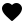
\includegraphics[scale=0.5]{figs/icons/icons8-heart-24.png} 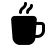
\includegraphics[scale=0.4]{figs/icons/icons8-coffee-cup-48.png}
    \end{itemize}
\end{frame}


\end{document}
